\section{Problem 1}

\subsection{Question}
\vspace*{10pt}
We know the group split in two different groups.  Suppose the
disagreements in the group were more nuanced -- what would the clubs
look like if they split into groups of 3, 4, and 5?
\clearpage
\subsection{Answer}
As was illustrated in the original study of Zachary's karate club, \cite{wzach77}, a prediction of the structure of the club if a separation were to occur can be made with a high degree of accuracy using weighted edges based on the perceived ``strength'' of each relationship it modeled. The prediction method outlined in the original paper was an implementation of the \textit{maximum flow-minimum cut labeling procedure} \cite{forful62}. The pickled \cite{py:pickle} dataset of the existing karate club, with weights for each edge, was obtained from \url{http://nexus.igraph.org/api/dataset_info?id=1&format=html} and used to create the graph shown in Figure \ref{fig:existing_graph}.

\begin{figure}[h!]
\centering
\fbox{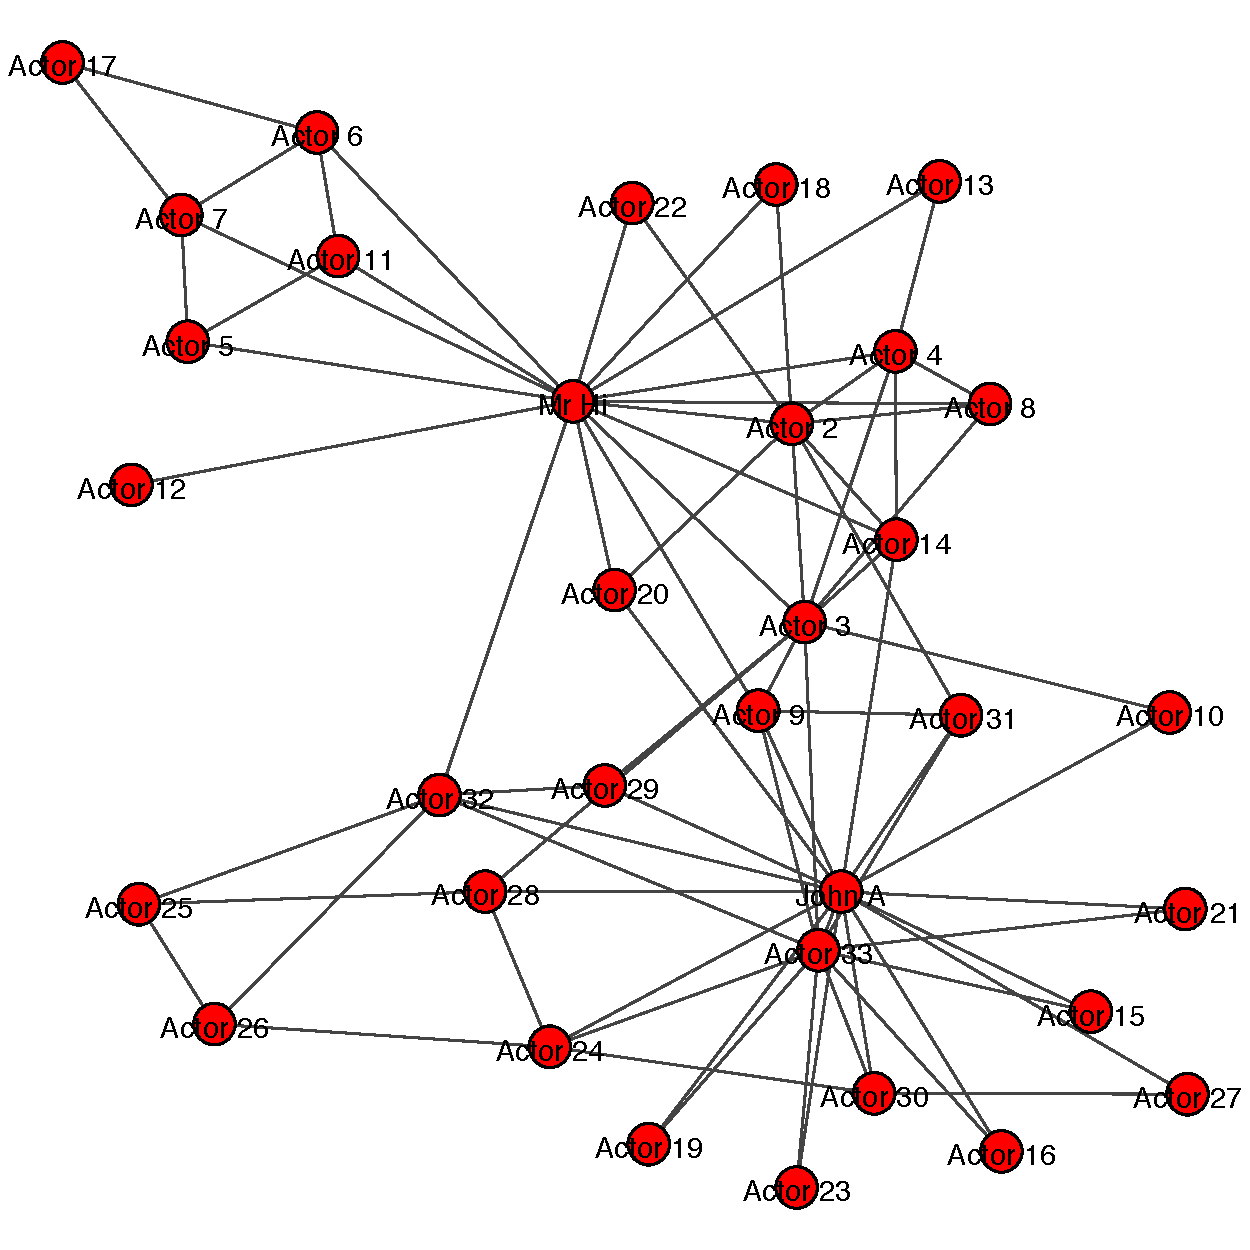
\includegraphics[scale=0.65]{q1/initial_karate_graph.pdf}}
\caption{The Existing Graph}
\label{fig:existing_graph}
\end{figure}

\clearpage

The actual structure of the two resulting clubs after the split are shown in Figure \ref{fig:actual}.

\begin{figure}[h!]
\centering
\fbox{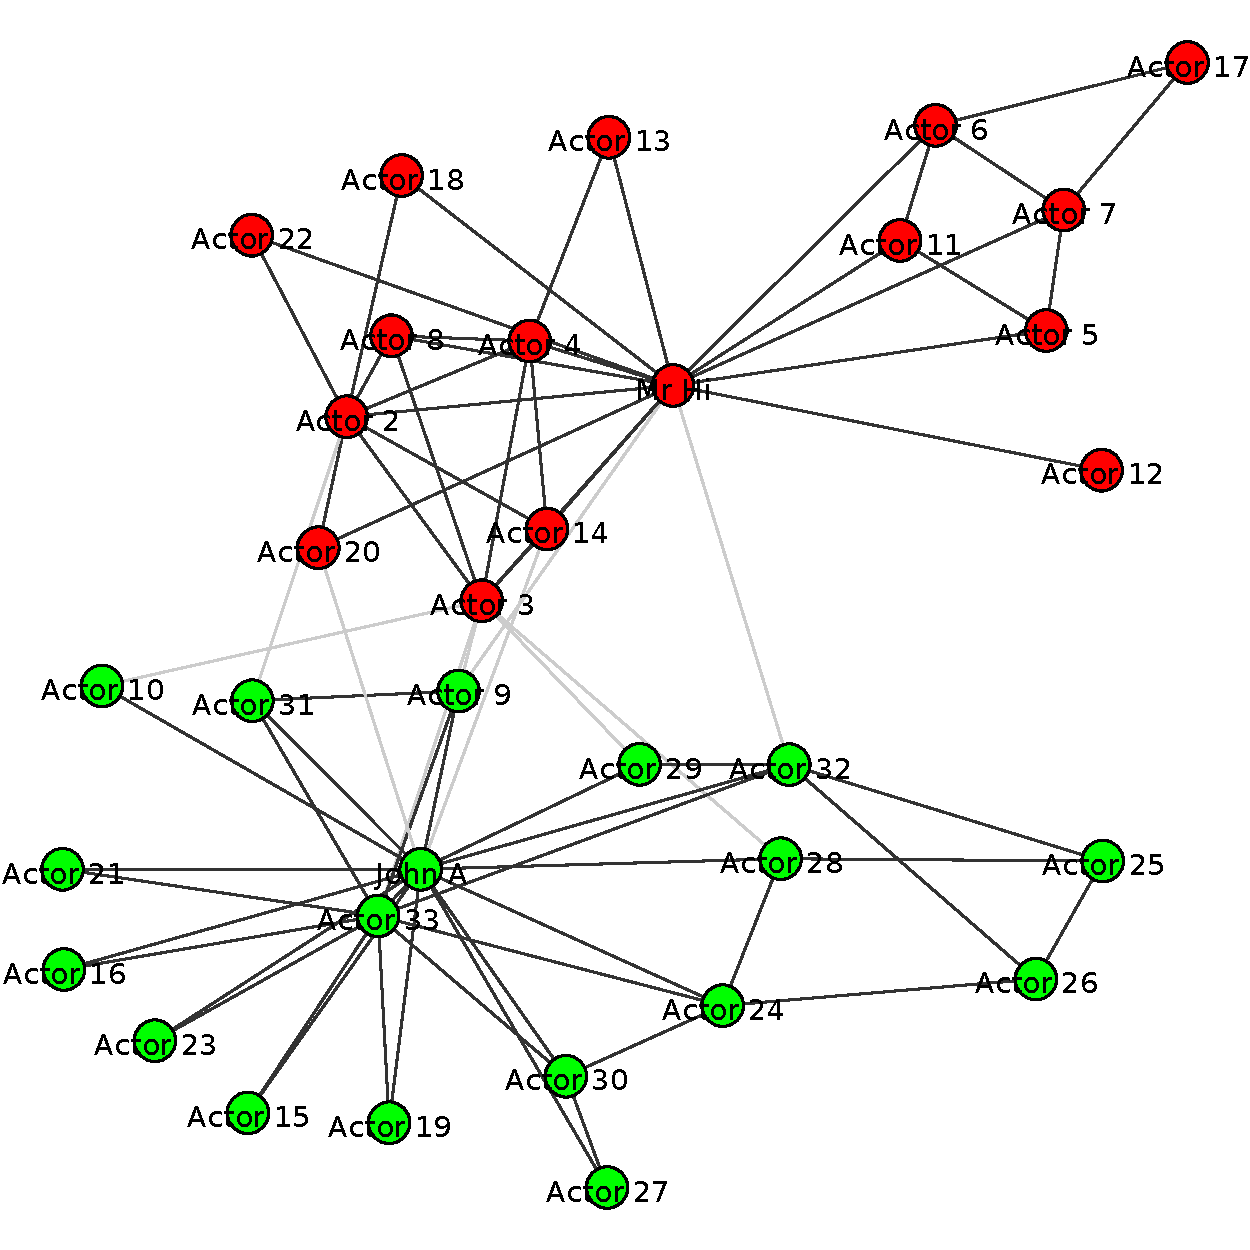
\includegraphics[scale=0.65]{q1/actual_after_split.pdf}}
\caption{Actual Graph After Split}
\label{fig:actual}
\end{figure}

To predict a separation of the existing graph into two or more distinct community components a pair of community detection algorithms will be employed and the results will be compared to the actual results of the split from Zachary's original study \cite{wzach77}. Community Detection was chosen as a means for predicting the results of fission events because it is logical that a given community would less likely be split along strong inter-community edges than those weaker, community-spanning edges.

\clearpage

The first algorithm used was the Edge Betweenness algorithm, developed by Girvan and Newman \cite{girnew04}. This is a divisive algorithm that removes edges that have the highest betweenness measure because these tend to be community-spanning edges. 

\begin{figure}[h!]
\centering
\fbox{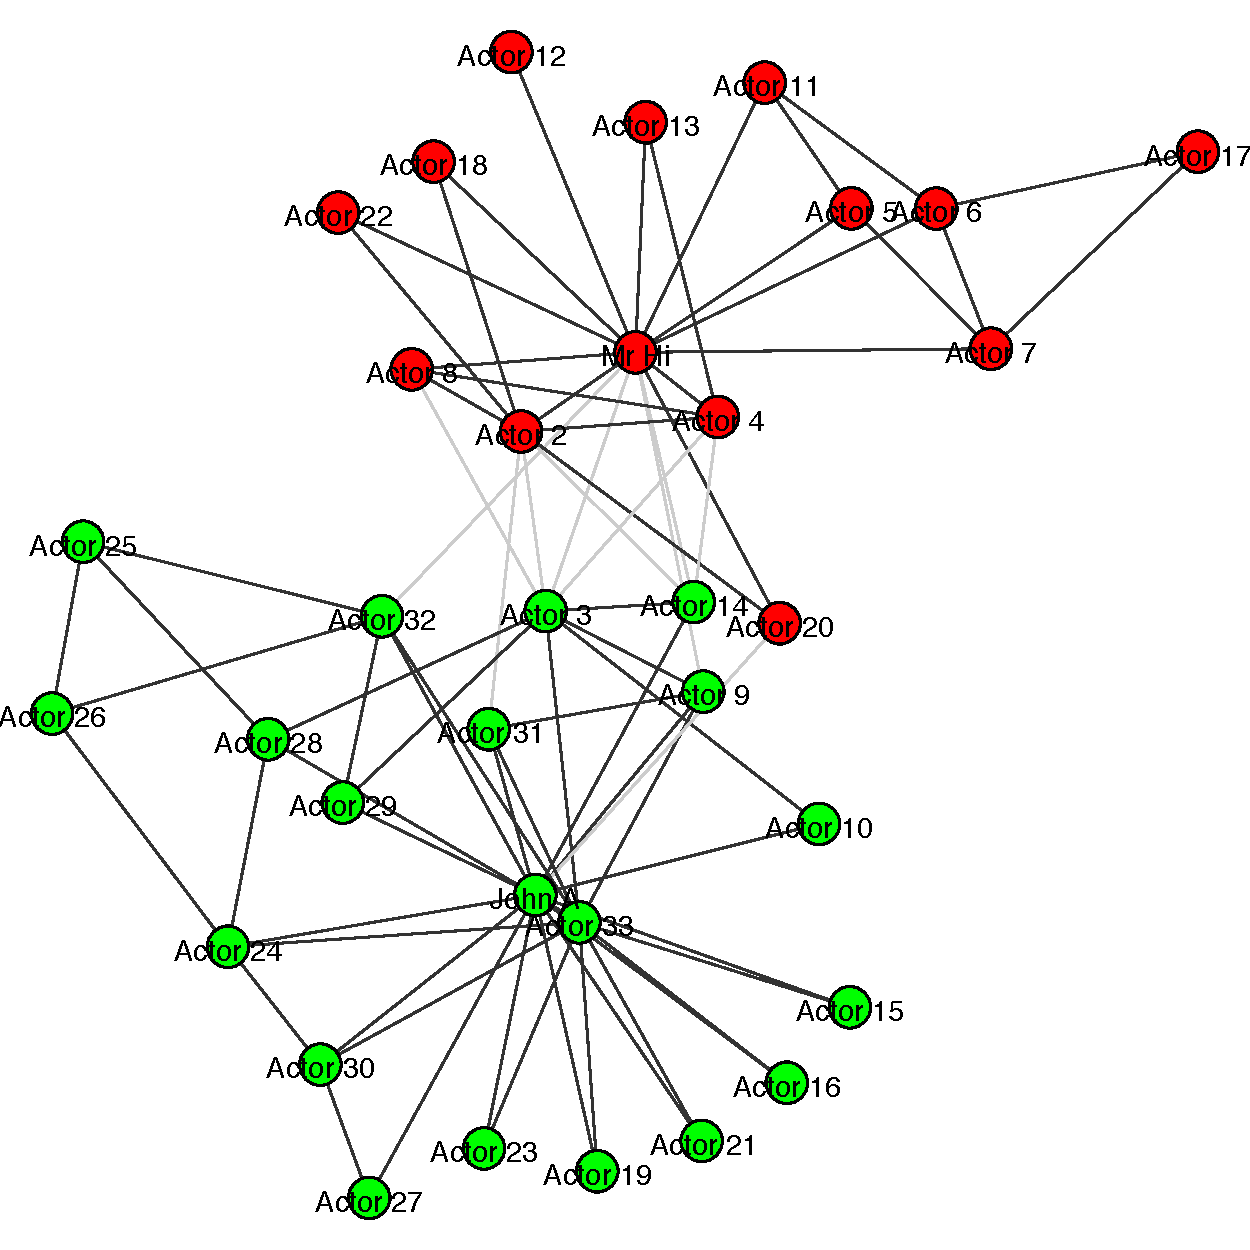
\includegraphics[scale=0.5]{q1/clust_eb.pdf}}
\caption{Prediction of Edge Betweenness Algorithm}
\label{fig:graph_eb}
\end{figure}

\begin{verbatim}
Edge Betweenness method results: 
Variant elements:
	[3, 14]
94.12% accuracy
\end{verbatim}

As you can see this method is fairly accurate, with over 94\% of the prediction being correct.
\\
My Girvan-Newman implementation has a $\frac{32}{34} = 94\%$ success rate, making it inferior in this case 
but still effective at predicting almost all of the group memberships. My implementation also predicted that individual $9$ would stay with Mr. Hi, which is the one membership that Zachary missed.

\clearpage

\begin{figure}[h!]
\centering
\fbox{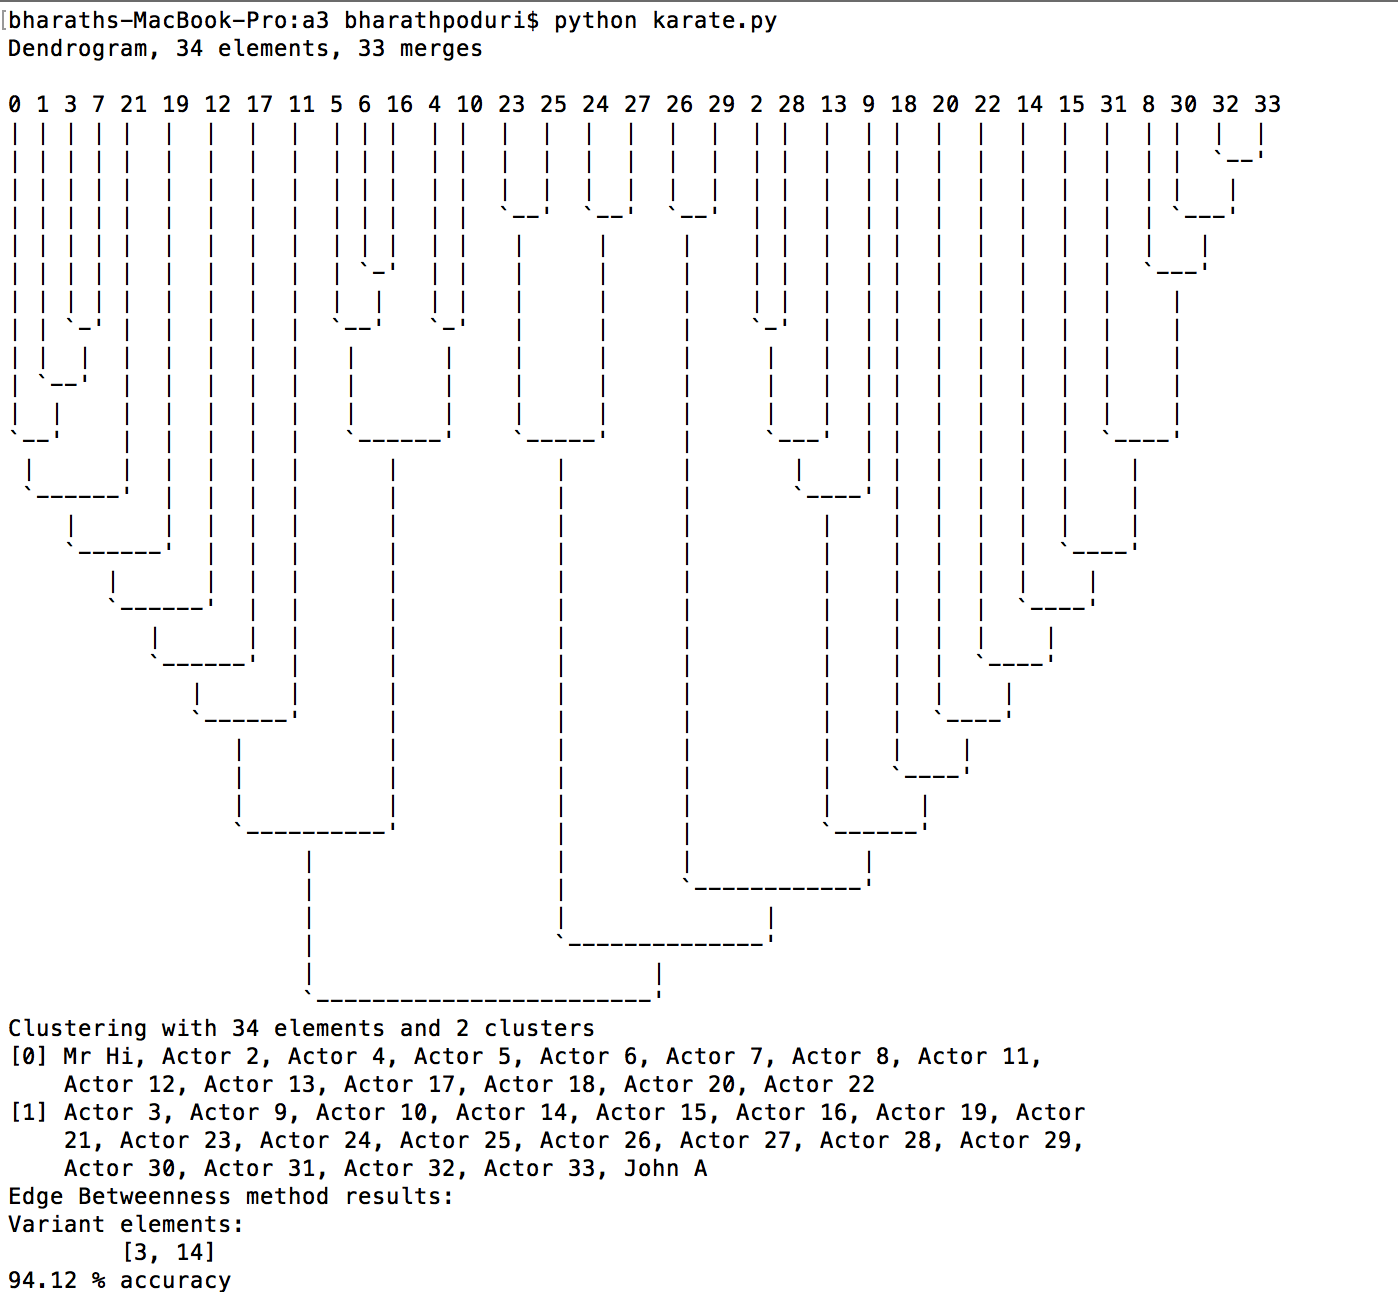
\includegraphics[scale=0.325]{q1/fig1.png}}
\caption{Dendrogram for Girvan-Newman}
\label{fig:output1}
\end{figure}

Table \ref{tab:results} shows the results compared with Zachary's original predictions and the actual data (\emph{Officers'} is John A's faction). Column 5 shows whether my Girvan-Newman implementation resulted in a \emph{Hit} (correctly calculated membership) or \emph{Miss} (incorrectly calculated membership).
\clearpage
\begin{table}
\centering
\small
\begin{tabular}{ | c | p{2cm} | p{2cm} | p{2cm} | p{2cm} | }
\hline
Individual & Actual Group\newline Membership From Split & Zachary's Ford and Fulkerson Procedure Modeled Group\newline Membership From Split & Girvan-Newman Modeled Group\newline Membership From Split & Hit/Miss For Girvan-Newman\\
\hline
1 & Mr. Hi & Mr. Hi & Mr. Hi & Hit \\
\hline
2 & Mr. Hi & Mr. Hi & Mr. Hi & Hit \\
\hline
3 & Mr. Hi & Mr. Hi & Mr. Hi & Hit \\
\hline
4 & Mr. Hi & Mr. Hi & Mr. Hi & Hit \\
\hline
5 & Mr. Hi & Mr. Hi & Mr. Hi & Hit \\
\hline
6 & Mr. Hi & Mr. Hi & Mr. Hi & Hit \\
\hline
7 & Mr. Hi & Mr. Hi & Mr. Hi & Hit \\
\hline
8 & Mr. Hi & Mr. Hi & Mr. Hi & Hit \\
\hline
9 & Mr. Hi & Officers' & Mr. Hi & Hit \\
\hline
10 & Officers' & Officers' & Mr. Hi & Miss \\
\hline
11 & Mr. Hi & Mr. Hi & Mr. Hi & Hit \\
\hline
12 & Mr. Hi & Mr. Hi & Mr. Hi & Hit \\
\hline
13 & Mr. Hi & Mr. Hi & Mr. Hi & Hit \\
\hline
14 & Mr. Hi & Mr. Hi & Mr. Hi & Hit \\
\hline
15 & Officers' & Officers' & Officers' & Hit \\
\hline
16 & Officers' & Officers' & Officers' & Hit \\
\hline
17 & Mr. Hi & Mr. Hi & Mr. Hi & Hit \\
\hline
18 & Mr. Hi & Mr. Hi & Mr. Hi & Hit \\
\hline
19 & Officers' & Officers' & Officers' & Hit \\
\hline
20 & Mr. Hi & Mr. Hi & Mr. Hi & Hit \\
\hline
21 & Officers' & Officers' & Officers' & Hit \\
\hline
22 & Mr. Hi & Mr. Hi & Mr. Hi & Hit \\
\hline
23 & Officers' & Officers' & Officers' & Hit \\
\hline
24 & Officers' & Officers' & Officers' & Hit \\
\hline
25 & Officers' & Officers' & Officers' & Hit \\
\hline
26 & Officers' & Officers' & Officers' & Hit \\
\hline
27 & Officers' & Officers' & Officers' & Hit \\
\hline
28 & Officers' & Officers' & Officers' & Hit \\
\hline
29 & Officers' & Officers' & Officers' & Hit \\
\hline
30 & Officers' & Officers' & Officers' & Hit \\
\hline
31 & Officers' & Officers' & Officers' & Hit \\
\hline
32 & Officers' & Officers' & Mr. Hi & Miss \\
\hline
33 & Officers' & Officers' & Officers' & Hit \\
\hline
34 & Officers' & Officers' & Officers' & Hit \\
\hline
\end{tabular}

\caption{Results of Split, as predicted by my Girvan-Newman Implementation and also compared to Zachary's predictions and the actual data}
\label{tab:results}
\end{table}


\clearpage

The second method used was the Leading Eigenvector algorithm developed by M. Newman \cite{new06}. This method uses a special matrix, called the modularity matrix, to determine which edges to remove.

\begin{figure}[h!]
\centering
\fbox{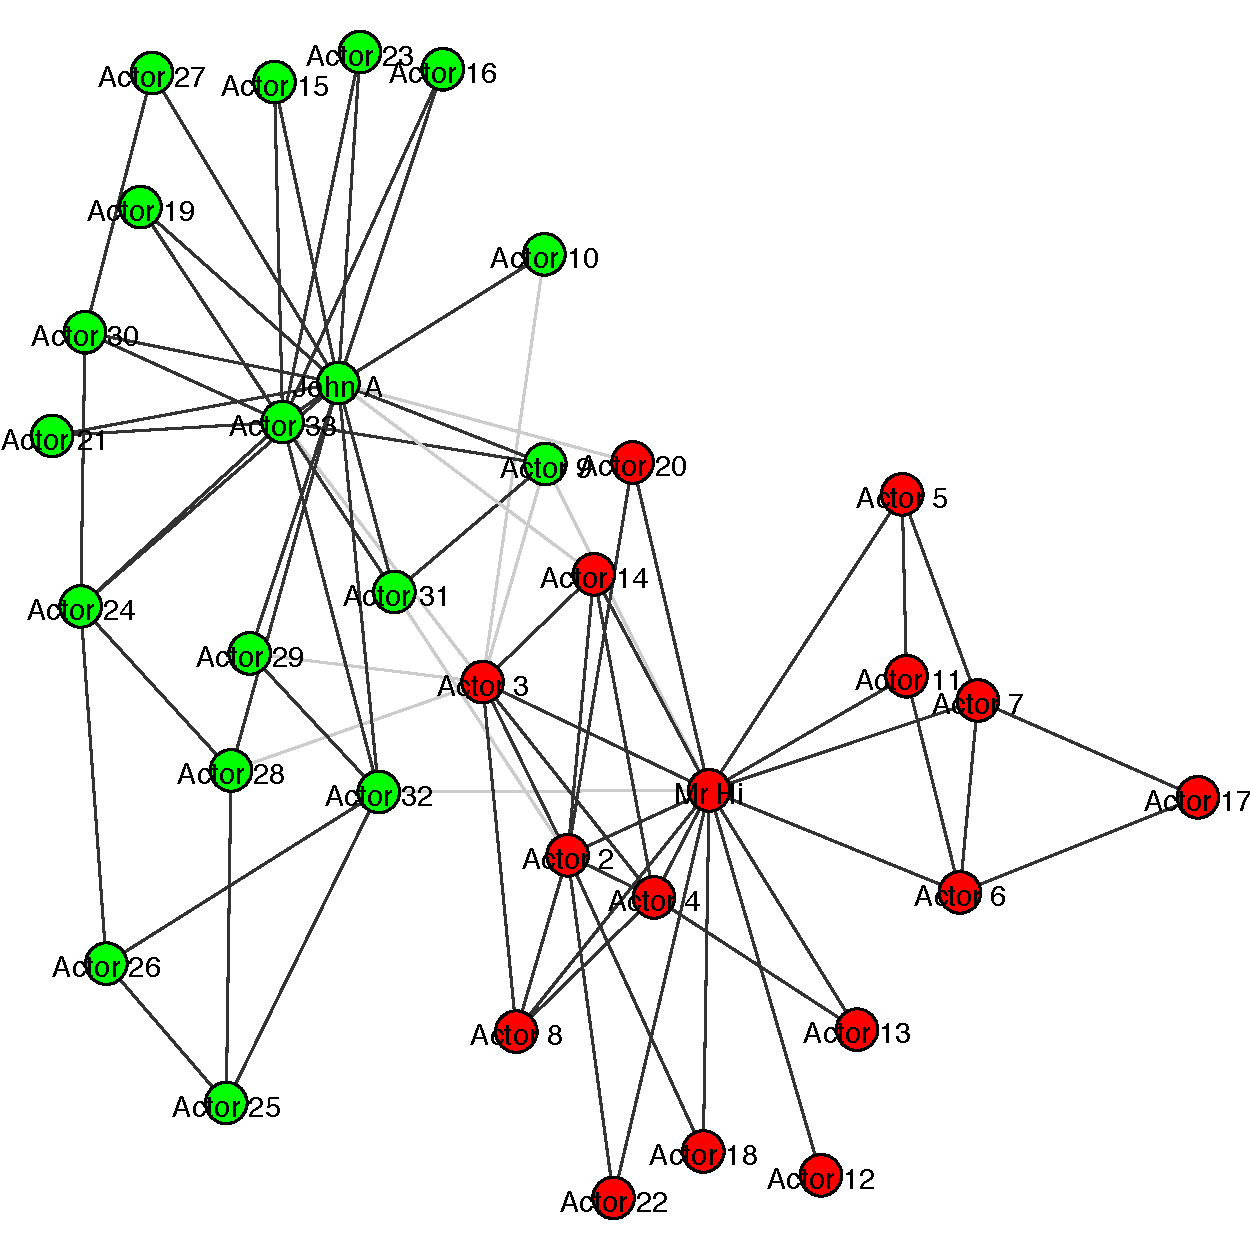
\includegraphics[scale=0.5]{q1/clust_le.pdf}}
\caption{Prediction of Leading Eigenvector Algorithm}
\label{fig:graph_le}
\end{figure}

\begin{verbatim}
Leading Eigenvector method results: 
Variant elements:
	[]
100.0 % accuracy
\end{verbatim}

This method proves 100\% efficacy in its prediction.

\begin{figure}[h!]
\centering
\fbox{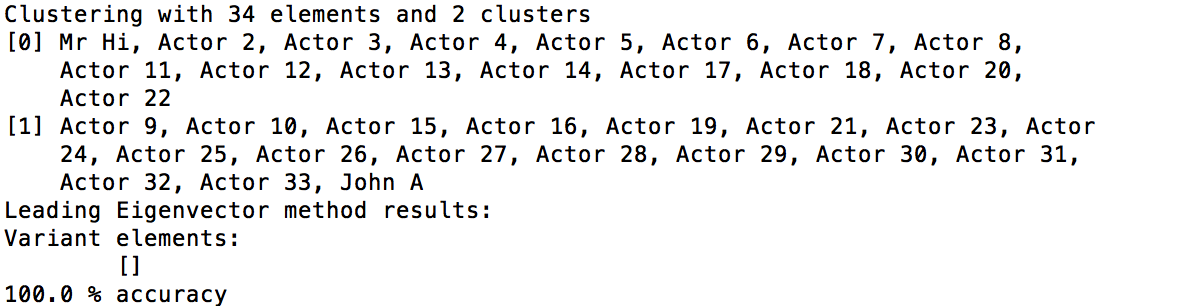
\includegraphics[scale=0.275]{q1/fig2.png}}
\caption{Leading Eigenvector method from Listing \ref{listing:karate}}
\label{fig:output2}
\end{figure}

\clearpage

The python code to produce these graphs is shown in Listing \ref{listing:karate}.

\lstinputlisting[language=Python, caption={Finding Communities in Zachary's Karate Club}, label=listing:karate]{q1/karate.py}